\begin{frame}{Generative models}{Linear discriminant analysis for $p > 1$}

\begin{itemize}
    \item We now extend the LDA classifier to the case of multiple predictors. \pause
    
    \item To do this, we will assume that $X = (X_1 , X_2 , \cdots , X_p )$ is drawn from a \textit{multivariate Gaussian distribution} \pause

    \item We assume that each individual predictor follows a one-dimensional normal distribution, with some correlation between each pair of predictors. \pause

    \item To indicate that a $p$-dimensional random variable $X$ has a multivariate Gaussian distribution, we write $X \sim N (\mu_k, \Sigma)$: \pause \\ $\rightarrow$ $\mu_k$ is a class-specific mean vector. \pause
    \\ $\rightarrow$ $cov(X) = \Sigma$ is common to all $K$ classes. \pause
    
    \item Formally, the multivariate Gaussian density is defined as \pause 

    \begin{equation}
        f(x) = \frac{1}{(2\pi)^{p/2} |\Sigma|^{1/2}} \text{exp } \left( -\frac{1}{2} (x-\mu_k)^T \Sigma^{-1} (x-\mu_k) \right) 
    \end{equation}
    
\end{itemize}
    
\end{frame}

\begin{frame}{Generative models}{Linear discriminant analysis for $p > 1$}

\begin{itemize}
    \item Plugging the density function $f_k (X = x)$, into (\ref{eq:bayes}), taking logs and performing a little bit of algebra reveals that the Bayes classifier assigns an observation $X = x$ to the class for which \pause

    \begin{equation}\label{eq:delta-linear-multi}
    \delta_k = x^T \Sigma^{-1} \mu_k - \frac{1}{2} \mu_k^T \Sigma^{-1} \mu_k + \log{(\pi_k)} 
    \end{equation}

    is largest. \pause \textcolor{blue}{This is the matrix version of (\ref{eq:delta-linear})} \pause

    \item The Bayes decision boundaries are the set
of values $x$ for which $\delta_k (x) = \delta_l(x)$ for $k \not= l$. \pause

    \item Once again, we need to estimate the unknown parameters $\mu_1 , \cdots , \mu_K$, $\pi_1 , \cdots , \pi_$ , and $\Sigma$. 

    \item The formulas are similar to those used in the one-dimensional case. 
    
\end{itemize}


\end{frame}

\begin{frame}{Generative models}{Linear discriminant analysis for $p > 1$}

\begin{columns}
    \column{0.5\linewidth}
    \footnotesize

    \begin{itemize}
    \item In a binary context, the Bayes classifier, and by extension LDA, uses a \textit{threshold} of 0.5 to assign an observation to a particular class. \pause

    \item But in some problems, this threshold is no longer optimal. \pause

    \item To help to decide which threshold value is the best, we can use the \textbf{ROC curve}. \pause

    \item The performance of the classifier, summarized over all possible thresholds, is given by the \textbf{Area Under the ROC Curve (AUC)}. \pause
    
\end{itemize}
    

    \column{0.5\linewidth}
        \onslide<3->{
        \begin{figure}[!h]
        \centering
        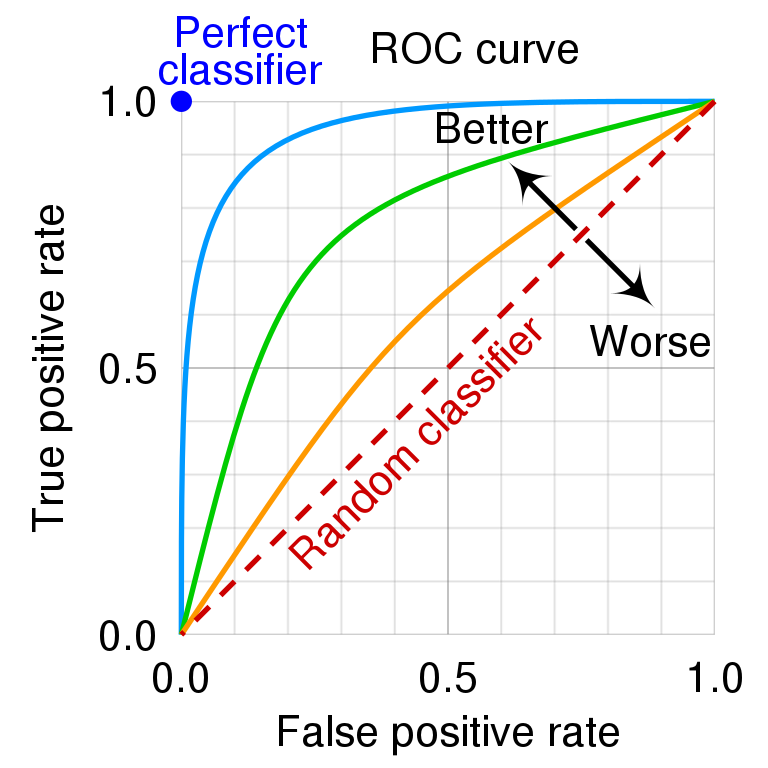
\includegraphics[width=4cm,height=4cm]{generative-models/roc-curve.png}
    \end{figure}} 
    \begin{itemize} \footnotesize
        \item An ideal ROC curve will hug the top left corner. \pause
        \item The larger the AUC the better the classifier.
    \end{itemize}

\end{columns}


\end{frame}
